\chapter{Implementación de $ISA^{2}$ con Swiftnet}
\label{ch:imp}
%TODO_DONE: Comentario general: una memoria de TFG no es un diario de trabajo. Debes tratar de reescribir ciertas partes, para que se haga una descripción técnica, y no parezca una guía paso a paso. Ambas cosas pueden convivir, y el documento puede/debe valer para que cualquiera repita paso a paso lo que has hecho, pero no puede parecer un diario de investigación.

%TODO_DONE Completar siguiente frase que resuma todo lo que vas a explicar en este capítulo
En este capítulo vamos a explicar cómo se ha implementado el sistema $ISA^{2}$ con Swiftnet resaltando aspectos como la creación de entornos \textbf{Conda} (\cite{conda}) y el uso de la librería \textbf{PyTorch} (\cite{pytorch}).

\section{Creación de entorno Conda e instalación de requisitos para Swiftnet}
A la hora de implementar esta nueva arquitectura debemos considerar que, para ejecutarla, hay que crear un entorno, un escenario, real sobre el que hacerlo. O, en su defecto, crear un entorno que simule esas condiciones para trabajar con ella.

Es por ello que antes de trabajar con el modelo de Swiftnet tenemos que sentar las bases sobre las que se pueda ejecutar. Así comienza la creación de un entorno Conda.

\textbf{Conda} (\cite{conda}) es un sistema de gestión de entornos con el que creamos el escenario sobre el que vamos a correr Swiftnet. Conda permite crear el escenario instalando y gestionando paquetes de uso público ubicados en diferentes \textbf{canales} del sistema. Simplemente hay que seguir las instrucciones que dan para descargarlos e instalarlos, y poder añadirlos así al escenario sobre el que se esté trabajando.

\begin{figure}[H]
  \centering
  
\includegraphics[width=8cm]{Figuras/Conda.eps}
  \caption{Conda}
\end{figure}

Antes de crear ningún entorno, primero hay que instalar Conda en la máquina con la que vamos a trabajar en este proyecto. Para ello descargamos \textbf{Miniconda} (un instalador de Conda) para Python 2.7 (\cite{miniconda_install}). Una vez descargado ya podemos crear entornos Conda.


Para crear el entorno Conda sobre el que trabajar basta con abrir un terminal del sistema operativo y escribir el siguiente comando:

\begin{center}
\textit{conda create --name swiftnet python=3.7}
\end{center}

En este caso estamos creando un entorno Conda llamado \textbf{swiftnet} con la versión de \textbf{Python 3.7}, que es la necesaria para el modelo Swiftnet, aunque se admiten versiones superiores  (\cite{github_swiftnet}). Y lo activamos con:

\begin{center}
\textit{conda activate swiftnet}
\end{center}

A continuación, descargamos el repositorio donde se encuentra el código de Swiftnet. Para ello basta con abrir una terminal del sistema operativo y ejecutar el siguiente comando en la carpeta donde se quiera extraer:

\begin{center}
\textit{git clone https:\textbackslash{}\textbackslash{github.com}\textbackslash{orsic}\textbackslash{swiftnet}}
\end{center}

Ya tenemos creado el entorno y hemos descargado el modelo, ahora hace falta añadirle los paquetes necesarios que requiere Swiftnet, indicados en el archivo \textbf{requirements.txt} del repositorio (\cite{github_swiftnet}). Para instalarlos simplemente seguimos las indicaciones del modelo y usamos este comando:

\begin{center}
\textit{pip install -r requirements.txt}
\end{center}

\textbf{Pip} (\cite{pip}) es otro gestor de paquetes que, junto a Conda, es muy útil a la hora de instalar aquellos paquetes que Conda no posee en sus canales.

Con el anterior comando, se instalan una serie de paquetes necesarios para la ejecución del modelo, entre ellos \textbf{PyTorch} (\cite{pytorch}), del cual hablaremos más adelante; pero no todos (en nuestro caso). Para que el modelo funcione correctamente hay que instalar los paquetes restantes con este comando (\cite{conda_sheet}):

\begin{center}
\textit{conda install nombre\_del\_paquete -c nombre\_del\_canal\_en\_el\_que\_se\_encuentra\_el\_paquete}
\end{center}

A continuación enumeramos los paquetes que quedan para poder ejecutar Swiftnet:

\begin{enumerate}
\item opencv (\cite{opencv})
\item pytorch torchaudio=0.4.0 cudatoolkit=10.0 (\cite{pytorch})
\item cython (\cite{cython})
\end{enumerate}

Cabe destacar que ponemos dichos paquetes con estas versiones porque las especificaciones de nuestra máquina así lo requerían. Si se quiere reproducir el resultado de este proyecto, puede que no sean las mismas versiones de estos paquetes los que haya que instalar, dependerá de la máquina sobre la que se trabaje.

Siguiendo con la operativa, pasamos a descargar la base de datos de Cityscapes sobre la que está entrenado Swiftnet para proceder a su utilización, tal y como describimos en la siguiente sección.

%TODO_DONE: En el párrafo siguiente faltan muchos detalles. Dí que hay que bajarse un repositorio, luego explica lo de las bases de datos paso a paso, ya qye recuerdo que había que descargarla y prepararla de una forma especial. Yo lo dejaría aquí todo bien documentado y explicado.

%TODO_DONE: mover esta subsección arriba tal y como te proponía,pero debes añadir muchos más detalles: imágenes, secuencias, info general de la base de datos, anotaciones, etc.
\subsection{Cityscapes}

Para la ejecución del modelo tomaremos como referencia la base de datos de Cityscapes (\cite{cityscapes}), como viene indicado en la guía de éste (\cite{github_swiftnet}), para poder comparar los resultados con los del paper de Swiftnet (\cite{swiftnet}).

Cityscapes es una base de datos que contiene imágenes de secuencias de vídeos en diferentes ciudades y escenarios. Descargaremos los siguientes archivos ``\textbf{.zip}'':

\begin{itemize}
\item \textbf{leftImg8bit\_trainvaltest.zip}
\item \textbf{gtFine\_trainvaltest.zip}
\end{itemize}

En el primero vienen tanto un set de imágenes preparadas para poder entrenar el modelo (\textbf{train}), como un set para evaluarlo (\textbf{val}) y otro para probarlo (\textbf{test}); nosotros nos quedaremos con los sets de evaluación y de entrenamiento (\textbf{val} y \textbf{train}).

En el segundo, hay información acerca de las máscaras de segmentación de las imágenes del primer archivo; viene en diferentes formatos y está organizado con el mismo sistema de carpetas de antes (\textbf{test}, \textbf{train} y \textbf{val}). Concretando para este segundo archivo, la información, en parte, viene dada en forma de anotaciones sobre las etiquetas que hay en las imágenes originales en archivos ``\textbf{.json}''. Más adelante concretaremos qué parte de ésta es necesaria para la correcta ejecución del modelo.

En la siguiente figura, se puede ver un ejemplo de cómo son ambos archivos:

\begin{figure}[H]
  \centering
    \begin{subfigure}[b]{0.45\linewidth}
    \includegraphics[width=\linewidth]{Figuras/Imagen_Cityscapes.eps}
    \caption{Imagen de Cityscapes (Primer archivo)}
  \end{subfigure}
    \begin{subfigure}[b]{0.45\linewidth}
    
\includegraphics[width=\linewidth]{Figuras/Mascara_Cityscapes.eps}
    \caption{Máscara de la imagen (Segundo archivo)}
  \end{subfigure}
      \begin{subfigure}[b]{0.45\linewidth}
    \includegraphics[width=\linewidth]{Figuras/Mascara_Color.eps}
    \caption{Máscara a color de la imagen (Segundo archivo)}
  \end{subfigure}
\end{figure}

Antes de continuar, es recomendable cambiar el nombre de las bases de datos que se han descargado de Cityscapes por nombres más sencillos por comodidad. En nuestro caso, llamamos \textbf{labels} a la carpeta que contiene las etiquetas de las imágenes (\textbf{gtFine\_trainvaltest}) y \textbf{rgb} a la carpeta que contiene las imágenes (\textbf{leftImg8bit\_trainvaltest}).

Cuando esté descargada la base de datos, vamos a la carpeta referente a las etiquetas (\textbf{labels}). Una vez dentro, tenemos que, o bien borrar todos los archivos \textbf{instanceIds} y \textbf{color}, o bien moverlos a otra carpeta. Esto es porque durante la ejecución del modelo, éste podría confundirse de archivos y coger los que queremos borrar (o mover), y nos interesa que utilice sólo los llamados \textbf{labelIds}. También aparecen unos archivos con la extensión \textbf{.json} que es conveniente dejarlos tal y como están.

Una vez hecho lo anterior, se sigue el procedimiento marcado por el modelo por el cual se guarda la base de datos de Cityscapes ya modificada en la carpeta \textbf{datasets} y una serie de modelos preentrenados para la misma en la carpeta \textbf{weights} (\cite{github_swiftnet}) y se ejecuta desde el directorio en el que éste se encuentra:

\begin{center}
\textit{python eval.py configs\textbackslash{rn18\_single\_scale.py}}
\end{center}

Tras ello, y en nuestro caso particular, se llegarán a dos errores:

\begin{enumerate}
\item No se encuentra el módulo \textbf{lib.cylib}.
\item No se encuentra la versión \textbf{GLIBCXX\_3.4.26} de \textbf{libstdc++} que se encuentra en el sistema operativo. A este último llegaremos más adelante, cuando hayamos modificado los archivos \textbf{rn18\_single\_scale.py} y \textbf{cityscapes.py}; sin embargo, este error puede no darse, todo dependerá de los medios de los que se disponga.
\end{enumerate}

Pasamos a explicarlos.

\subsection{Error de lib.cylib}

Este error se da porque aún no se ha creado un módulo de \textbf{cython} (\cite{cython}) necesario para evaluar las métricas del modelo. Se consigue ejecutando el código del archivo \textbf{build.sh} que se encuentra en la carpeta \textbf{lib} de éste.

Sin embargo, antes de ejecutarlo conviene modificarlo de la siguiente manera, tal y como mostramos en la Figura \ref{fig:cylib}:

\begin{figure}[H]
  \centering
  \includegraphics[width=12cm]{Figuras/cylib.eps}
  \caption{Archivo build.sh con las modificaciones necesarias para el compilado.}
  \label{fig:cylib}
\end{figure}

Tras hacerlo, lo ejecutamos con el siguiente comando:

\begin{center}
\textit{.\textbackslash{build.sh}}
\end{center}

Si nos sale algún error porque falta algún paquete por instalar, volvemos al comando que utilizamos para instalar paquetes por Conda y los instalamos de forma sencilla.

Como se puede observar en la figura \ref{fig:cylib}, el archivo está en \textbf{Shell Script} (\cite{shell}) y a través de éste se crean los archivos \textbf{cylib.so}, \textbf{cylib.cc} y \textbf{cylib.html}, necesarios para la ejecución del modelo.

Cabe destacar otra observación muy importante en la figura: Hay que modificar las líneas en las que se hace referencia al sistema de archivos propio de la máquina sobre la que se trabaja.

En nuestro caso, tenemos la siguiente ruta seguida de los directorios que se han creado al haber instalado \textbf{Conda} y los paquetes previos a la ejecución del modelo:

\begin{center}
\textit{\textbackslash{home}\textbackslash{sergios}\textbackslash{miniconda2}\textbackslash{envs}\textbackslash{swiftnet}}
\end{center}

Es muy importante cambiar esa ruta por la de la máquina sobre la que se trabaje, si no, no puede funcionar; de modo que cuando se instale Conda y se cree el entorno sobre el que se quiere trabajar, hay que tener muy en cuenta dónde se instala para modificarla.

Por otro lado, el resto de la ruta no se cambia, ya que son paquetes comunes a cualquier usuario que intente ejecutar Swiftnet (\cite{swiftnet}).

Por último, puntualizar que la última parte comentada del archivo, que es muy similar a la que hemos modificado hace un momento, sirve para lo mismo pero utilizando \textbf{Python 3.8}. Si se quisiese utilizar este modelo con esa versión de Python habría que descomentarla y comentar la referente a Python 3.7. Lo demás se mantendría como está.

\subsection{Error de GLIBCXX}

Para empezar, \textbf{libstdc++} (\cite{glibcxx}) es la implementación de la librería estándar del lenguaje \textbf{C++} de programación.

Esto quiere decir que para cualquier programa en C++ que use hilos o archivos, por ejemplo, usará esta librería para implementar lo pertinente a estas cosas en las librerías de C++.

Por otro lado tenemos la \ac{ABI}, la cual sirve para que, por ejemplo, un programa compilado en libstdc++ en 2013 funcione de la misma manera para una nueva versión de libstdc++ en 2021. Cuando se actualiza esa librería y se quiere compilar un programa de una versión anterior, se mantiene la \ac{ABI} de dicha versión para compilar ese programa (\cite{glibcxx}).

Sin embargo, cuando se actualiza libstdc++ y se mantiene su \ac{ABI}, cada función o símbolo de dicha librería obtiene una nueva versión, a la que llamamos mediante un \textbf{linker}.

El linker enlaza la llamada a una función de la librería con su última versión (\cite{glibcxx}).

Para nuestro caso, no encuentra la versión \textbf{GLIBCXX\_3.4.26} de \textbf{libstdc++} debido a que el linker no tiene permisos para acceder a la librería del sistema operativo. Por lo que, cada vez que ejecutemos el modelo, aunque lo intente, no podrá encontrar dicha librería.

Sin embargo, he aquí una razón de uso de los entornos Conda: cuando se crea un entorno Conda nuevo, éste también adquiere esta librería al venir incluida en uno de los paquetes de instalación predeterminados para la creación del entorno. De este modo obtenemos la versión que requiere Swiftnet para su ejecución.

Aún así sigue existiendo un problema: el linker sigue buscando la versión requerida por Swiftnet en el mismo lugar, de modo que cada vez que se llame a esa librería el linker seguirá buscando donde siempre y seguiremos igual. La solución reside en hacerle saber al linker dónde buscar esta nueva versión, y para ello usaremos este comando en la terminal:

\begin{center}
\textit{export LD\_LIBRARY\_PATH=\$LD\_LIBRARY\_PATH:\$HOME\textbackslash{miniconda2}\textbackslash{lib}\textbackslash{}}
\end{center}

No obstante, esta solución sirve siempre y cuando no se cierre la terminal. En el momento en el que se cierre hay que volver a abrir otra y volver a utilizarlo.

Al usarla, conseguimos nuestro objetivo y podemos seguir avanzando en la ejecución del modelo.

\section{PyTorch}

Anteriormente lo hemos mencionado, y a diferencia de otros paquetes de instalación, éste conviene explicarlo más en detalle, pues es la librería para \textbf{deep learning} en la que se basa Swiftnet para hacer la \ac{SS}.

\begin{figure}[H]
  \centering
  
\includegraphics[width=8cm]{Figuras/PyTorch.eps}
  \caption{PyTorch}
\end{figure}

\textbf{PyTorch} (\cite{pytorch}) es un framework de Python de \textbf{deep learning} que permite su utilización en aplicaciones que implementan visión por computador o IA. Está basado en la librería \textbf{Torch}, de ahí que los paquetes que se requieren instalar por Conda tengan el mismo nombre y derivados.

PyTorch trabaja, entre otras cosas, con \textbf{tensores}, que sirven para operar con \textbf{arrays de n-dimensiones}. Este tipo de variables se usan durante todo el modelo de Swiftnet ya que son las que obtendrán, por ejemplo, la lectura de datos de las imágenes, la información de las etiquetas (persona, vehículo, \ldots).

En esencia, PyTorch posibilita la existencia del modelo de Swiftnet. Si no se utilizase, podríamos utilizar otros como \textbf{Tensorflow} (\cite{tensorflow}) o \textbf{Caffe} (\cite{caffe}), sin embargo, cada uno de estos frameworks está enfocado hacia diferentes aspectos y habría que analizar cuál de ellos podría ser el adecuado para el modelo. 

PyTorch se puede instalar tanto para máquinas con tarjeta gráfica como sin ella, dependiendo de cómo se quiera ejecutar. Generalmente, se suele instalar en máquinas con tarjeta gráfica y por ello se instala, además de los paquetes de Torch, el paquete \textbf{cudatoolkit}. Este paquete interactúa con \textbf{CUDA} (\cite{cuda}).

\subsection{CUDA}

CUDA (\cite{cuda}) es una plataforma desarrollada por \textbf{NVIDIA} para poder trabajar, a nivel de cómputo, con las \ac{GPU}s.

Como ya hemos dicho, el paquete \textbf{cudatoolkit} es necesario para trabajar con PyTorch en máquinas con tarjeta gráfica (\ac{GPU}). Sin embargo, es posible instalarlo y poder ejecutar PyTorch sin la \ac{GPU}, es decir, a través de la \ac{CPU}.

Basta con hacerle saber a PyTorch sobre qué ejecutarlo con la siguiente instrucción:

\begin{center}
\textit{torch.device('cpu'/'gpu')}
\end{center}

Escribiendo dicha instrucción en el código que se quiera ejecutar especificando una de las dos opciones que se dan (\ac{CPU} o \ac{GPU}), podemos obligar a PyTorch a que trabaje con una u otra. El uso de esta instrucción es meramente opcional, ya que para los medios que tenemos disponibles no es necesaria, pero puede ser útil mencionarla si se diera el caso opuesto.

En cuanto a términos de rendimiento, es recomendable, si es posible, que PyTorch trabaje con una \ac{GPU}, puesto que al hacerlo de la otra forma, la carga de procesos que tendría que soportar la \ac{CPU} sería elevada y conllevaría a que tardase demasiado la ejecución del modelo. Con \ac{GPU}, sin embargo, sería más veloz y podríamos trabajar con mayor soltura al no tener largos tiempos de espera durante la ejecución de Swiftnet.


\section{Swiftnet}

Ya hemos explicado las bases sobre las que se sustenta Swiftnet (PyTorch y CUDA) y sobre dónde ejecutarlo (entorno Conda), además de explicar y solucionar los errores que pueden ocurrir durante el proceso. A continuación pasamos a explicar el propio modelo y cómo ejecutarlo paso a paso.
\subsection{Pycharm}

Para ejecutar Swiftnet nos hemos ayudado de un \ac{IDE} llamado \textbf{Pycharm} (\cite{pycharm}).

Pycharm nos sirve para poder comprobar la ejecución del modelo paso a paso. De otra manera, si lo hiciéramos desde la terminal, resultaría mucho más difícil saber cómo procesa las imágenes. Se puede descargar de manera muy sencilla.

\subsection{Proceso de Swiftnet}
En este TFG antes de aplicar el modelo Swiftnet a las imágenes de la base de datos $ISA^2$, quisimos asegurarnos de que todo funcionaba correctamente, intentando replicar los resultados que se ofrecen en el artículo de Swiftnet sobre la base de datos Cityscapes. Es por ello que detallamos todo este proceso en esta memoria.

Así pues, una vez tenemos Pycharm podemos pasar a ejecutar Swiftnet, el cual funciona de la siguiente manera:

\begin{enumerate}
\item En primera instancia, Swiftnet carga las especificaciones del archivo de configuración \textbf{rn18\_single\_scale.py} que pasaremos a modificar a continuación.
\item Más adelante, carga la información de las etiquetas (persona, carretera, vehículo, \ldots).
\item A continuación, carga el modelo de \ac{SS} que se va a utilizar con CUDA (\cite{cuda}).
\item Por último, evalúa el modelo cargado usando las imágenes de la base de datos de Cityscapes, la información de las etiquetas, \ldots  Para evaluarlo sigue los siguientes pasos:

\begin{itemize}
\item Crea una pila para guardar las predicciones que se van a hacer de las imágenes de Cityscapes. Con \textbf{predicciones} nos referimos a \textbf{imágenes segmentadas por el modelo}.
\item En la pila creada, se colorizarán las etiquetas de las predicciones y se formarán éstas. En esencia, la pila será la encargada de realizar estas funciones además de guardar los resultados en el directorio adecuado.
\item Una vez se crea la pila, se crean lotes de imágenes que van a pasar por el modelo para que éste los vaya segmentando. Es decir, el modelo va a ir etiquetando las imágenes del lote según las clases que detecte en las mismas.
\item Una vez todo finaliza, se calcula el porcentaje de acierto que ha tenido el modelo con las imágenes reales. De ahí se extraen los datos que aparecen en el paper de Swiftnet.
\end{itemize}   
\end{enumerate}
Sin embargo, si lo ejecutamos siguiendo el comando que nos dice el procedimiento del modelo no funcionará.

Esto es porque antes de ejecutarlo debemos modificar el archivo \textbf{rn18\_single\_scale.py} de la carpeta \textbf{configs}. En este archivo, hay que cambiar lo siguiente:

\subsection{Archivo rn18\_single\_scale.py}

\begin{enumerate}
\item Cambiar el valor de la variable \textbf{evaluating} a \textbf{True} en la línea 22.
\item Modificar dos rutas en las líneas que se detallan:
\begin{itemize}
\item \textbf{'datasets'} en la línea 18
\item \textbf{'weights\textbackslash{rn18\_single\_scale}\textbackslash{model\_best.pt}'} en la línea 70
\end{itemize}

Básicamente hay que modificarlas poniendo la \textbf{ruta absoluta} en cada una de ellas para asegurarnos de que, al ejecutar el modelo, encuentre los archivos de éstas; indicando además en la primera el directorio de la base de datos de Cityscapes.

\item Añadir la siguiente instrucción en la línea 45 del archivo (opcionalmente se puede añadir en la línea 57, pero sólo si se quisiese entrenar el modelo, cosa que no haremos puesto que no es necesario):

\begin{center}
\textit{RemapLabels(Cityscapes.map\_to\_id, Cityscapes.num\_classes)}
\end{center}

Esta última es de vital importancia para el funcionamiento de Swiftnet. Cuando ejecutemos Swiftnet y no pongamos esta instrucción, cada vez que analice las etiquetas de una imagen se confundirá. Esto es porque cuando Swiftnet obtiene las etiquetas de Cityscapes (\textbf{data\textbackslash{cityscapes}\textbackslash{labels.py}}), filtra sólo las que le son necesarias.

Cada una de ellas viene identificada por un número (por ejemplo, la clase \textbf{carretera} tiene asociado el número 7). De este modo, cuando filtra las etiquetas, por cómo accede a ellas para saber cual es cual, obvia estos números y las identifica por el orden en que se han filtrado.

Tomando el ejemplo de la clase \textbf{carretera}: Si esta clase tiene asociado el número 7, y ha sido filtrada en primer lugar, aunque el modelo detecte que en una imagen hay píxeles de la clase \textbf{carretera} (con el número 7), para él ``\textbf{carretera}'' tendrá el número 0 por ser la primera clase filtrada.

Con la instrucción anterior evitamos ese tipo de errores.
\end{enumerate}

Por último, debemos modificar un último archivo para poder replicar los resultados de Swiftnet. En el siguiente capítulo los presentaremos y explicaremos en detalle.
%TODO_DONE: hay que añadir los resultados aquí, o decir, si se ha hecho así, que los presentarás en el capítulo X

Para que funcione Swiftnet, nos vamos al directorio \textbf{data} del modelo, y a su vez nos dirigimos al que lleva por nombre \textbf{cityscapes}, para modificar el archivo \textbf{cityscapes.py}.

\subsection{Archivo cityscapes.py}

Este archivo es el responsable de obtener las imágenes de la base de datos de Cityscapes pero si no hacemos los siguientes cambios no cumplirá con lo establecido:

\begin{enumerate}
\item \textbf{home = Path.home()} en la línea 5.

Esta instrucción crea una variable llamada \textbf{home} que contendrá la ruta hacia el directorio homónimo.

\item \textbf{self.root = home} en la línea 41.

Inicializamos la variable \textbf{self.root} con el valor de la variable \textbf{home} antes creada.

\item \textbf{self.images\_dir = self.root \textbackslash{} 'Desktop' \textbackslash{} 'swiftnet' \textbackslash{}'datasets' \textbackslash{} 'Cityscapes' \textbackslash{} 'rgb' \textbackslash{} subset} en la línea 42.

Cambiamos la ruta por donde va a obtener las imágenes de Cityscapes.

\item \textbf{self.labels\_dir = self.root \textbackslash{} 'Desktop' \textbackslash{} 'swiftnet' \textbackslash{} 'datasets' \textbackslash{} 'Cityscapes' \textbackslash{} labels\_dir \textbackslash{} subset} en la línea 43.

Cambiamos la ruta por donde va a obtener las etiquetas de Cityscapes.

\item \textbf{self.images = list(sorted(self.images\_dir.glob('*\textbackslash{*.png}')))} en la línea 48.

Obtenemos una lista ordenada de archivos \textbf{.png} de la base de datos de Cityscapes y la guardamos en la variable \textbf{self.images}.
\end{enumerate}

\subsection{Evaluación final en Cityscapes}

Para concluir con una evaluación de resultados de segmentación semántica en Cityscapes, basta con ejecutar el modelo con la instrucción:

\begin{center}
\textit{python eval.py configs\textbackslash{rn18\_single\_scale.py}}
\end{center}

Si hemos hecho todo bien, obtendremos los mismos resultados que en el paper de Swiftnet (\cite{swiftnet}) en la carpeta \textbf{out} del directorio \textbf{configs} (las imágenes vendrán en formato \textbf{``.jpg''}).

Cuando veamos las imágenes segmentadas, veremos que aparecen la imagen real procesada en primer lugar, la imagen segmentada a continuación, y por último la máscara de segmentación de la imagen real mostrándonos las etiquetas originales para poder obtener el \ac{IoU} de cada una y el \ac{mIoU} final (cite{miou-iou}). En el siguiente capítulo explicaremos estas métricas.

Esto se puede cambiar en el archivo \textbf{prediction.py} de la carpeta \textbf{evaluation}. He aquí un ejemplo del resultado original y del resultado modificado:

\begin{figure}[H]
\centering
  \begin{subfigure}[b]{0.45\linewidth}
    \includegraphics[width=\linewidth]{Figuras/Imagen_Concatenada.eps}
    \caption{Resultado Original}
  \end{subfigure}
  \begin{subfigure}[b]{0.45\linewidth}
    \includegraphics[width=\linewidth]{Figuras/Imagen_Modificada.eps}
    \caption{Resultado Modificado}
  \end{subfigure}
  \caption{Resultados}
  \label{fig:img_con}
\end{figure}
%TODO_DONE: añade una imagen de ejemplo

En dicho archivo, dentro de la clase \textbf{StorePreds}, en el método \textbf{call}, ponemos la siguiente instrucción:

\begin{center}
\textit{store\_img = np.concatenate([i.astype(np.uint8) for i in [self.to\_color(p)]], axis = 0)} en la línea 25
\end{center}

Con esa simple modificación podemos ver únicamente la imagen segmentada en los resultados.

\section{Ejecutando Swiftnet sobre $ISA^{2}$}
%TODO_DONE: todo lo que viene aquí hay que sacarlo de esta subsección y ponerlo en esta sección. Cambia el texto e introduce el problema, ahora vamos a contar nuestra implementación, ya no hay más configuraciones de entorno, ni pruebas de métrica con el paper de switnet

Sin embargo, nuestro trabajo no lo hemos realizado con la base de datos de Cityscapes, sino con la de $ISA^{2}$ (\cite{isa2}). Para hacerlo con esta nueva base de datos simplemente hay que:

\begin{itemize}
\item Cambiar las rutas de la base de datos de Cityscapes y sustituirlas por las de $ISA^{2}$ en el archivo \textbf{rn18\_single\_scale.py}, en las líneas que modificamos.
\item Comentar las líneas 77, 79, 82 del archivo \textbf{evaluation\textbackslash{evaluate.py}}.
\item Modificar el archivo \textbf{cityscapes.py} de la siguiente manera:

\begin{enumerate}
\item Tras la instrucción \textbf{self.root = home} hay que poner \textbf{self.subset = subset}
\item \textbf{self.images\_dir = self.root \textbackslash{} 'Desktop' \textbackslash{} 'swiftnet' \textbackslash{} 'datasets' \textbackslash{} 'ISA2'} en la línea 42.
\item Comentar las líneas en las que se inicializan las variables \textbf{self.labels\_dir} y \textbf{self.depth\_dir}.
\item \textbf{self.images = list(sorted(self.images\_dir.glob('*\textbackslash{*}\textbackslash{*.jpeg}')))} en la línea 48
\item Comentar las líneas 65 y 66
\end{enumerate}

\item Por último, modificar la clase \textbf{StorePreds} del archivo \textbf{prediction.py} en la carpeta \textbf{evaluation} siguiendo las instrucciones:

\begin{enumerate}
\item \textbf{import scipy.io} en la línea 3
\item \textbf{from scipy.io import savemat} en la línea 4
\item Cambiar la instrucción de la línea 28 por la siguiente:
\begin{center}
\item \textit{scipy.io.savemat(f'{self.store\_dir}\textbackslash{ISA2}\textbackslash{{name}.mat}', {''name'': name, ''data'' : p})}
\end{center}
\end{enumerate}

Con estas modificaciones tan sencillas podemos trabajar con la base de datos de $ISA^{2}$. En nuestro caso, hemos hecho multitud de modificaciones en esos archivos para automatizar el modelo, es decir, guardar todas las imágenes procesadas en sus correspondientes carpetas. Sin embargo, lo hemos hecho por comodidad y no es necesario hacerlo; con las instrucciones anteriores es suficiente para ejecutar el modelo correctamente.

Cabe destacar que en el archivo \textbf{prediction.py}, siguiendo las figuras, se puede ver la llamada a un método llamado \textbf{savemat}. Éste sirve para guardar las imágenes segmentadas en archivos \textbf{``.mat''} que en el siguiente paso utilizaremos, de modo que, aunque no es estrictamente imprescindible, sí es recomendable usarlo puesto que nos resultará mucho más fácil manejar las imágenes segmentadas en los códigos de \textbf{MatLab} (\cite{matlab}) si están en ese formato.

\end{itemize}

Ejecutando el modelo de nuevo con la anterior instrucción, obtendremos los resultados para esta nueva implementación:

\begin{center}
\textit{python eval.py configs\textbackslash{rn18\_single\_scale.py}}
\end{center}

Si obtenemos los resultados de la misma forma que con Cityscapes (\ref{fig:img_con}), basta con modificar el archivo \textbf{prediction.py} de la carpeta \textbf{evaluation} de la misma forma que antes.

En la clase \textbf{StorePreds} del archivo \textbf{prediction.py}, en el método \textbf{call}, ponemos la siguiente instrucción:

\begin{center}
\textit{store\_img = np.concatenate([i.astype(np.uint8) for i in [self.to\_color(p)]], axis = 0)} en la línea 25
\end{center}

Así obtendremos los resultados del modelo con esta nueva implementación, de una forma clara y concisa.

Aquí acaba todo lo pertinente a Swiftnet. Hemos visto cómo ha segmentado las imágenes y el proceso interno que lo hace posible, además de trabajar con dos bases de datos. El siguiente paso es la realización de histogramas de las imágenes segmentadas y su posterior introducción en los sistemas de regresión para estimar la velocidad adecuada. Todo ello se hará en \textbf{MatLab} (\cite{matlab}).

\section{Obtención de histogramas basados en la segmentación semántica}

En este apartado vamos a detallar cómo obtener los histogramas en función de los datos de segmentación semántica, que son las características de entrada a los modelos de regresión para predecir la velocidad adecuada a cada imagen, tal y como se describe en el sistema $ISA^{2}$.

Un histograma es una representación gráfica en forma de barras que simboliza la distribución de un conjunto de datos (\cite{histograma}). En nuestro caso, nuestros histogramas representan el porcentaje que hay de cada etiqueta en una imagen. He aquí un ejemplo de un histograma genérico:

\begin{figure}[H]
  \centering
  \includegraphics[width=8cm]{Figuras/histograma.eps}
  \caption{Histograma}
\end{figure}

Para realizar los histogramas reutilizamos los códigos de $ISA^{2}$ de MatLab de la primera versión. Puesto que los resultados de Swiftnet están en el mismo formato que los de DeepLab, apenas hay que modificar los códigos.

Simplemente hay que actualizar las rutas para que recoja los resultados de Swiftnet y no de DeepLab.

Aplicando estos cambios obtenemos unos archivos en formato \textbf{``.mat''} (como los resultados de Swiftnet), que contienen los histogramas correspondientes a cada imagen de cada subcarpeta de la base de datos de $ISA^{2}$.

Es en este punto del proyecto en el que se utiliza la técnica de \ac{SPP} (\cite{spp_real}) de la que hablábamos en un principio para generar el descriptor de imagen que, posteriormente, se pasará a cada uno de los sistemas de regresión. En el siguiente paso, se volverá a utilizar para comprobar la efectividad de estos sistemas para 4 niveles de agrupación (\textbf{pooling}), es decir, añadiendo más información en el descriptor dependiendo del nivel de \ac{SPP} que se utilice (\cite{isa2}).

Previo a continuar es necesario recordar \ac{SPP} y su importancia en la realización del proyecto.

Como ya explicamos en el capítulo \ref{ch:isa2}, \ac{SPP} se basa en la concatenación de histogramas generados para diferentes niveles de subdivisión de la imagen dependiendo del nivel de agrupación que se quiera utilizar. Como resultado se obtiene un vector final (o descriptor) que codifica la información espacial de los píxeles de la imagen.

En otras palabras, según el nivel de agrupación a utilizar, \ac{SPP} aplicará más o menos subdivisiones de la imagen, y por ende se obtendrán en consecuencia histogramas con información más o menos precisa, es decir, con mayor o menor nivel de granularidad. De este modo, con \ac{SPP} conseguimos los descriptores de imagen necesarios para aplicarlos en los sistemas de regresión que ahora explicamos.

%En primera instancia, \ac{SPP} se utiliza para construir el descriptor de imagen, situándose para ello tras las capas convolucionales de la \ac{CNN}. Así, \ac{SPP} recoge los mapas de características (de un tamaño cualquiera y provenientes de las imágenes de entrada) procesados por las capas convolucionales de la \ac{CNN} (en el caso de Swiftnet, \textbf{ResNet-18} \cite{swiftnet}), y los divide en un número de ``compartimentos espaciales'' (\textbf{Spatial Bins}) con un tamaño proporcional al de la imagen de entrada \cite{spp2}. Estos compartimentos vendrán dados con diferente granularidad, es decir, con distinto nivel de detalle.

%Dependiendo del nivel de agrupación que se quiera usar habrá mayor o menor granularidad y, por ende, habrá mayor o menor información para el descriptor de imagen. Cuando se procese el descriptor en los sistemas de regresión, la estimación será más fiel a la realidad conforme aumente el nivel de agrupación, aunque de esto hablaremos en el siguiente capítulo.

%TODO_DONE: te dejo comentados los párrafos anteriores porque están mal, debes mirar la descripción que he hecho del SPP en el fichero anterior y añadirla aquí, ya que lo que tienes es incorrecto. Espero que ahora ya sepas lo que es el SPP. Lo has confundido con otro técnica, con el mismo nombre, que se emplea en CNN.

\section{Sistemas de regresión}

Pasamos a explicar los diferentes sistemas de regresión que hemos aplicado en este proyecto para comprobar cuánta mejoría hay con respecto a la primera versión de $ISA^{2}$ (\cite{isa2}).

Los sistemas de regresión sirven para calcular una estimación de la velocidad en cada imagen y compararla con la velocidad real a la que deberían ir los vehículos según la situación de la vía. Con cada uno de ellos aplicamos un nivel diferente de \textbf{pooling} (\ac{SPP}), como hemos explicado anteriormente, para comparar entre ellos cuál es más eficiente a través del \ac{MAE} (\cite{mae}).
 
El \ac{MAE} es la métrica que usamos para establecer con qué sistema trabaja mejor el proyecto. Se basa en calcular la media de la diferencia absoluta de los valores reales con los valores de predicción de la velocidad. Como se puede ver en la siguiente fórmula, \textit{X} es una matriz con los valores reales e \textit{Y} es una matriz con los valores de predicción.

\begin{equation}\label{eq:MAE}
MAE = \frac{\sum_{i=1}^{n}|X_i - Y_i|}{n}
\end{equation}

Más adelante veremos una serie de figuras en las que se verá representado.

%TODO_DONE Añade fórmula.

En cuanto a los modelos de regresión empleados en nuestra evaluación para sistemas $ISA^2$, pasamos a explicar nociones básicas de cada uno de ellos, sin entrar en mucho detalle.
%TODO_DONE: para cada una de ellas añade la función de MATLAB que se emplea, y comenta sus parámetros de entrada.
\subsection{Regresor Lineal}

La regresión lineal (\cite{linear}) es un tipo de análisis predictivo usado de forma muy común siendo uno de los más básicos que existen. Se utiliza para explicar la relación entre una variable predictiva (independiente) y otra variable de salida (dependiente). La siguiente ecuación es la forma más simple de expresar esta relación:

\begin{equation}
y = c + b*x
\end{equation}

Siendo \textit{y} la variable de salida (dependiente), \textit{c} una constante, \textit{b} el coeficiente de regresión y \textit{x} la variable predictiva (independiente).

Para este tipo de regresión usaremos la siguiente instrucción en MatLab:

\begin{center}
\textit{fitlm(X,Y)}
\end{center}

Con ella entrenamos un modelo de regresión lineal con las matrices de datos \textit{X} e \textit{Y} (\cite{fitlm}), siendo \textit{X} la matriz correspondiente al descriptor de imagen que se generó previamente e \textit{Y} la matriz correspondiente a la velocidad apropiada para dicha imagen.

\subsection{Lasso}

La regresión \textbf{Lasso} (\cite{lasso}) es un tipo de regresión lineal que hace uso de la \textbf{contracción} (\cite{shrinkage}). Con la contracción conseguimos que valores extremos de una muestra se reduzcan alrededor de un valor central como, por ejemplo, la media. Este tipo de regresión viene bien para modelos con altos niveles de \textbf{multicolinealidad}, es decir, con una fuerte correlación entre variables predictivas o explicativas (\cite{multicollinearity}).

Usaremos la siguiente instrucción:

\begin{center}
\textit{lasso(X,Y,'Alpha',1,'CV',10)}
\end{center}

Con estos parámetros, se realiza la regresión regularizada (\cite{lasso-matlab}) usando el método de red elástica (\cite{elasticnet}) con el parámetro \textit{Alpha} a 1 y la validación cruzada (\cite{cv}) de 10 veces. Ambos campos \textit{X} e \textit{Y} representan lo mismo que en el sistema anterior.

\subsection{Boosting Trees}

Este tipo de sistema se basa en dos algoritmos (\cite{boosting-trees}):

\begin{itemize}
\item Algoritmos de \textbf{árboles de decisión}.
\item Métodos de \textbf{boosting}.
\end{itemize}

El objetivo de usar algoritmos de árboles de decisión es crear un modelo \textbf{entrenado} que se pueda usar para predecir el valor de una variable, a través de una serie de reglas de decisión que le sirvan a dicho modelo para \textbf{aprender} a decidir, construidas en base a unos datos de \textbf{entrenamiento} (\cite{decision-tree}).

Por otro lado, tenemos los métodos de \textbf{boosting}. En esencia, el boosting es una manera de conseguir un sistema más robusto combinando los resultados (decisiones) de los árboles de decisión (\cite{boosting}).

Con esta instrucción (\cite{fitrensemble}) lo llevaremos a cabo:

\begin{center}
\textit{fitrensemble(X,Y,'NumLearningCycles',numTrees,'Learners',t,'KFold',5,'LearnRate',learnRate(k))}
\end{center}

Según ésta, se realiza la regresión usando, para ello, las matrices \textit{X} e \textit{Y} junto con los parámetros \textit{NumLearningCycles} (Número de árboles de decisión), \textit{Learners} (Número máximo de \textbf{splits}, es decir, ramificaciones en el árbol), \textit{KFold} (Validación cruzada) y \textit{LearnRate} (Parámetro de aprendizaje del sistema).

Con todo ello tendremos un sistema de regresión final que, por lo general, suele dar buenos resultados, tal y como se muestra en \cite{isa2}.

\subsection{SVR}

El sistema \ac{SVR} es una variante del sistema \ac{SVM} para realizar regresión (\cite{SVR}). Se trata de una adaptación del modelo de clasificación básico, implementado por las máquinas de vectores soporte, para conseguir que estas implementen una solución de regresión.

Se consigue usando esta instrucción (\cite{fitrsvm}) en nuestro código de MatLab:

\begin{center}
\textit{fitrsvm(X,Y,'KernelFunction', 'linear', 'KernelScale', 'auto')}
\end{center}

Los parámetros usados (ademas de las matrices \textit{X} e \textit{Y}) son: \textit{KernelFunction}, que sirve para entrenar el sistema usando una función kernel (Método de entrenamiento) \textit{linear}, como viene especificado en la instrucción; y \textit{KernelScale}, que sirve para determinar el parámetro de escala del núcleo (en nuestro caso, con valor \textit{auto}, es decir, mediante un proceso heurístico).

%Hemos detallado todo el proceso del sistema de $ISA^{2}$, junto a su implementación, en diferentes bloques. Cada uno de los bloques ha sido explicado según la relevancia que ha tenido durante la ejecución del proyecto y según los problemas que ha podido dar en el mismo, con su posterior solución.

%A continuación vamos a mostrar los resultados finales de cada uno de los sistemas de regresión, utilizando tanto figuras como tablas.

